\chapter{Developing the tool}
This chapter details how the visualization tool was built.

\section{Creating the tiles}
The tiles got created using a modified version of gdal2tiles, which was changed to create tiles following the XYZ format. However, since the default output bit depth is too low, it would have to be modified further. The file format would also have to be changed to tiff in order to be visualized with the geotiff.js library. 

\subsection{Changing the file type}
Changing the file format can be done by changing two lines in the gdal2tiles script:

\begin{lstlisting}[language=iPython, caption={Changing the file format}, label= VoresPY,escapechar=|]
#Original code
#self.tiledriver = 'PNG'
#self.tileext = 'png'
#New code
self.tiledriver = 'GTiff'
self.tileext = 'tiff'
\end{lstlisting}
This changes the raster driver from png to the geotiff format and the file extension from png to tiff. 
\citep{RasterDrivers}
The geospatial information, which is the difference between a geotiff and a regular tiff, gets lost in process. This information is not important for this project since the tiles are being loaded based on their name and folder placement, not based on the internal metadata.

Running gdal2tiles with these changes will produce a tiff file, which still would be limited to 8 bits. 
\subsection{Increasing the bit depth}
The reason for the bit limit is that gdal2tiles uses the memory dataset driver, which have 8 bits as default.  This default can overwritten to 32 bits by adding “gdal.GDT\_Int32” to every instance where the driver is being used as demonstrated in code x. 
\citep{MoreThan8}

\begin{lstlisting}[language=iPython, caption={Increasing the bit depth}, label= VoresPY,escapechar=|]
self.mem_drv = gdal.GetDriverByName('MEM')
...
#Old code
#dstile = mem_drv.Create('', tile_size, tile_size, tilebands)
#New code
dstile = self.mem_drv.Create('', self.tilesize, self.tilesize, tilebands, gdal.GDT_Int32)
\end{lstlisting}
The memory driver is being used four times, which all have been changed in a similar fashion.


The script is now generating tiff tiles correctly. However it also generates KML files for visualization in Google Earth, which is undesired since it would increase the processing time and required storage space. 
\subsection{Prevent generation of Google Earth files}
gdal2tiles is automatically generating KML files if the projection is EPSG:4326. According to the documentation for the official gdal2tiles this can be disabled with the command "--no.kml".
\citep{gdal2tilesDoc}


This command does not prevent the creation of the files in the modified version. Therefore the automatic generation has been removed from the code. This was done by commenting out the lines shown in x. 

\begin{lstlisting}[language=iPython, caption={Increasing the bit depth}, label= KML,escapechar=|]
 if self.out_srs and srs4326.ExportToProj4() \
         == self.out_srs.ExportToProj4():
     self.kml = True
     self.isepsg4326 = True
     if self.options.verbose:
         print('KML autotest OK!')
\end{lstlisting}
        

\fxnote{Write about the addition to time the whole thing}


\subsection{Command for tile creation}

After all the modification are in place the script can be run by running the command illustrated below:


python <path to modified gdal2tiles script> --leaflet --zoom=<desired zoom levels> --profile=raster --webviewer=none <input file> <output directory>


Most of these inputs are from the documentation for the original gdal2tiles, though the leaflet command is from the modified version. This command ensures that tiles are being created following the XYZ formatting instead of the TMS. The zoom command defines which zoom levels should be generated. An example of an input could be 0-2, which would generate tiles for the zoom levels 0, 1 and 2. 

Setting the profile to raster was done because the two other options (mercator and geodetic) resulted in the error message "list index out of range", while the raster profile gave a useable product. The selection of this options and its consequences is expanded upon in section x.  

The webviewer option prevent the generation of webviewers to visualize the tiles. These default webviewers is created to visualize tiles of the original format, so they would be unable to visualize the modified tiles. 
The input file is the name of the processed file and output directory is the folder, where the tiles get created. 
\subsection{Result}

While creating the tiles the error message "ERROR 1: Buffer too small" gets displayed. The tiles are still being generated with the correct formatting and bit depth. This is an error message from numpy, which gdal2tiles are using. 
\citep{MoreThan8}
The generated tiles appears as they should, so this error message is potentially referring to the geospatial information, which gets lost.

The tiles at the rightmost and bottom edges have an edge as shown in figure x. This edge is not being shown, when the tile is being loaded into the map. A comparison between the input file and the tile shows that all data is being displayed. The bottom part of the input file is the last part before the edge. This edge seems to be generated because the input file was not perfectly dividable with the tile size as illustrated in figure x.
https://github.com/ARiisgaard/Thesis/issues/22
This edge could be another explaination for the error message. 



\fxnote{Make figures - remove link}


\fxnote{Test if normal gdal2tiles tiles have edges - if false, then point it out here}

The script also produces an xml file with metadata. An example of the content of said metadata file can be seen in code x.

\begin{lstlisting}[language=HTML5, caption={The metadata from the xml file generated by the modified gdal2tiles}, label= VoresHTML,escapechar=|]
<?xml version="1.0" encoding="UTF-8"?>
<TileMap tilemapservice="http://tms.osgeo.org/1.0.0" version="1.0.0"><Abstract/><SRS>GEOGCS["WGS 84",DATUM["WGS_1984",SPHEROID["WGS 84",6378137,298.257223563,AUTHORITY["EPSG","7030"]],
AUTHORITY["EPSG","6326"]],PRIMEM["Greenwich",0,AUTHORITY["EPSG","8901"]],UNIT["degree",0.0174532925199433,
AUTHORITY["EPSG","9122"]],AXIS["Latitude",NORTH],AXIS["Longitude",EAST],AUTHORITY["EPSG","4326"]]
</SRS><BoundingBox maxy="25.00000000000814" maxx="80.99999999999989" miny="19.00000000000815" minx="72.99999999999989"/><Origin y="19.00000000000815" x="72.99999999999989"/><TileFormat extension="tiff" mime-type="image/tiff" height="256" width="256"/><TileSets profile="raster"><TileSet order="2" units-per-pixel="0.00833333333333" href="2"/><TileSet order="3" units-per-pixel="0.00416666666667" href="3"/><TileSet order="4" units-per-pixel="0.00208333333333" href="4"/><TileSet order="5" units-per-pixel="0.00104166666667" href="5"/><TileSet order="6" units-per-pixel="0.00052083333333" href="6"/><TileSet order="7" units-per-pixel="0.00026041666667" href="7"/><TileSet order="8" units-per-pixel="0.00013020833333" href="8"/><TileSet order="9" units-per-pixel="0.00006510416667" href="9"/></TileSets></TileMap>
\end{lstlisting}


\fxnote{How long time did it take to run?}

Running it parallelly it parallelly 

\section{Visualizing tiles}
After the tiles got created, they are stored in a folder, which gets uploaded to the testserver along the index file. 
The metadata from the xml file must be loaded into the map to be able to visualize the tiles. Normally this could be done using the WMTSCapabilities() function in Openlayers.
\citep{WmtsOl}
However, the formatting of the xml file produced by gdal is different from the format, which this function can read. Therefore, a small script has been created to parse the xml file and store the information in a metadata object. This object, tileMetadata, stores the bounding box, origin, center coordinates as well as tilesize. The initial version of the object also stored the resolution data, which is called units-per-pixel in code x. This led to some inconsistency when loading tiles, which had been generated without some of the lower zoom level. This will be further expanded upon in section x. Therefore, the resolution was instead generated using the script x, where 0.0333 is the value for units-per-pixel at zoom level 0. 

\begin{lstlisting}[language=JavaScript, caption={The JavaScript in the project}, label= VoresJS,escapechar=|]
for (var z = 0; z < 14; ++z) {
// generate resolutions and matrixIds arrays for this WMTS
//The number in the resolution calculation is the units-per-pixel value at zoomlayer 0 in the xml file generated by gdal2tiles
resolutions[z] = 0.03333333333514 / Math.pow(2, z);
matrixIds[z] = z;
}
\end{lstlisting}
Using this metadata, the tiles could be visualized using the olGeoTiff class. 

%\begin{lstlisting}[language=JavaScript, caption={The JavaScript in the project}, label= VoresJS,escapechar=|]
%var wmslayer = new ol.layer.Tile({
%  source: new ol.source.WMTS({
%    url: tileFolders + '/{TileMatrix}/{TileCol}/{TileRow}.tiff',
%    projection: projection,
%    tileGrid: new ol.tilegrid.WMTS({
%      origin: tileMetadata[origin],
%      resolutions: resolutions,
%      matrixIds: matrixIds,
%      tileSize: tileMetadata[tileSize],
%    }),
%    requestEncoding: 'REST',
%    transition: 0
%  }),
%  extent: tileMetadata[boundingBox],
%  opacity: 0.65 
%});
%var olgt_map = new olGeoTiff(wmslayer);
%\end{lstlisting}


\subsection{Custom colors scheme}
Using colorbrewer a custom sequential colorscheme was generated. This scheme was added to Plotty and selected as a color palette.
*This code might change a bit, so wait with writing  


\section{Loading data at a wrong resolution}\label{PresentingBug}
Figure x shows how the map looked, when loaded with a manually defined max value.


\begin{figure} [H]
	\centering
	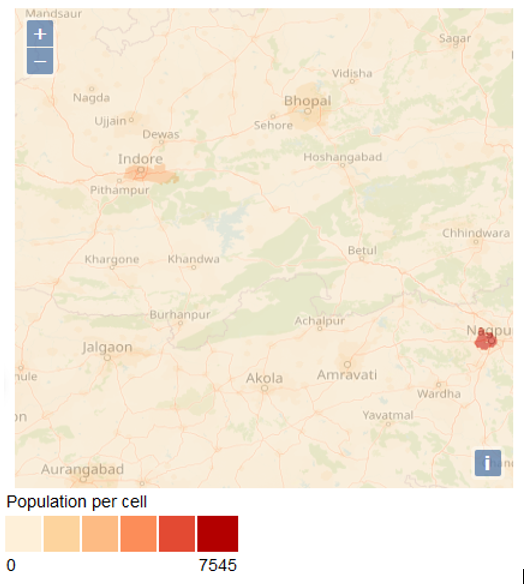
\includegraphics[width=.8\textwidth]{Pictures/MapWithWrongResolution}
	\caption{The map looking right, but with tiles from the wrong zoom level}
	\label{MapWithWrongResolution}
\end{figure}


While the map appeared to look alright, it was loading tiles from the wrong zoom level. The tiles always got loaded from a zoom level 3 lower than intended. So the map in figure x is visualizing the map at zoom level 7 but loading and displaying tiles from zoom level 4.

Some experiments with loading the tiles from the correct zoom level 
Setting up Openlayers to download tile from the current view and correct zoom level chrashed the map with the error message “Insufficient Resources”. The amount of loaded tiles seems unnecessarily high and size of the tiles too small. This seems to indicate, that the tiles, which the modified version of gdal2tiles associates with zoom level 7 in fact belongs to a higher zoom level.

The reason for this bug was never discovered and the bug never got fixed. When the resolution data was gathered from the metadata file, the difference between the loaded and the actual zoom level would between different sets of tiles. This variance would depend on the which zoom levels were not being generated. So, if only the zoom levels 2-7 were generated, the difference would increase by one for each missing layer. In this case the loaded tiles would instead be wrong by 5, calculated as the default wrongness of 3 plus 2 for missing zoom layer 0 and 1. 
This bug will be defining for the rest of the code.



\section{Calculate max value in current extent}
Calculating the highest value in the current extent can be divided into two smaller tasks. Figuring out which tiles currently are being displayed and processing these tiles.

\subsection{Current displayed tiles}

The tiles, which currently is within the view, can be found using the Openlayers tileGrid method forEachTileCoord. This method can trigger a function for each tile within a given zoom level and extent. 
\citep{forEachTileCoord}
The method is going through the tiles based on their coordinates, but this can be translated to the tile urls using the getTileUrlFunction.
\begin{lstlisting}[language=JavaScript, caption={The JavaScript in the project}, label= VoresJS,escapechar=|]
var tileUrlFunction = wmslayer.getSource().getTileUrlFunction()
var zoomlevelAdjustment = 3
wmslayer.getSource().getTileGrid().forEachTileCoord(loadExtent, mapZoom - zoomlevelAdjustment, function(tileCoord) {
	tileName = tileUrlFunction(tileCoord, ol.proj.get('EPSG:4326'))
	%Find max value
}
\end{lstlisting}
forEachTileCoord is triggering for each tile in the given zoom extent. This means that it on zoom level 7 it would load the tiles, that should be rendered on zoom level 7. Due to the bug mentioned section \ref{PresentingBug} it is not the tiles from that zoom level, which are being displayed. Instead the tiles from zoom level 2 are being displayed. This will complicate some of the next steps. 
The adjustment to the zoom level is in order to load the tiles, which should have displayed.

\subsection{Max value for each tile}
If the tiles added to the map had been from the correct zoom level calculating max value of a tile could have been done as olGeoTiff were running. olGeoTiff holds the values for the tiles in a dataarray already, so finding the maximum value could be done with a single line adding a tiles max value to the dictionary for that tile. This line is shown in code x, where urlToTiff is the name of the object, which holds the data.
maxValueTileData[url].maxValue = Math.max(...urlToTiff[url][0])
However, since olGeoTiff holds data from an incorrect zoom layer this would not function. A possible solution would be to trigger forEachTileCoord for the same wrong zoom layer as the displayed tiles are from. This solution was not implemented since it would result in a map with could potentially so misleading information. The explanation for this has been illustrated in figure x. 

Todo: Figure with showing how large the loaded tiles are compared with how large they should be.

The tiles from the wrong zoom level are so large, that they would show data outside the view of the map. This means that the coloring could be based on the information that was outside of the current view.

The alternative solution is to run another function going through the tiles, which should have been displayed and find the highest value among these. This would result in a map where the wrong tiles were being colored based on information from the smaller correct tiles. This solution is by no means ideal. It means requesting tiles from two layers, one for displaying on the map a one for calculating the relevant max values. Loading more data than necessary will make the script slower, but since no better solution was not found this have been implemented.
The calculation of the maximum value for each tile was done in a very similar fashion to how olGeoTiff operates as illustrated in figure \ref{CalculateMaxValue}. An object holds information about all tiles, which have been processed and the max value is known. When the function is run for a tile it first checks if the tile already has been processed. If that is not the case, then it will create an object for the data, which it then will load and parse with geotiff.js. The data array with parsed data will then be run through as descripted in code x to calculate the maximum value. This maximum value will then be returned to the map. 


\begin{figure} [H]
	\centering
	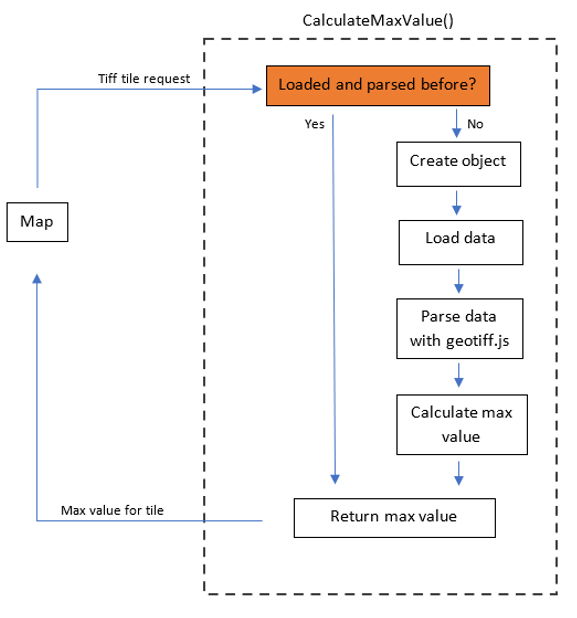
\includegraphics[width=.8\textwidth]{Pictures/CalculateMaxValue}
	\caption{Flow diagram of the calculation over max value in a tile}
	\label{CalculateMaxValue}
\end{figure}



\subsection{Highest tile value the current displayed}


To find the largest tile value among all the currently displayed tiles forEachTileCoord as mentioned earlier is used. forEachTileCoord does not have a trigger for when it has run through all the tiles. This functionality is necessary for ensuring that the produced maximum value is actually the maximum value. Without a precise end trigger the coloring applied to the map could be based on the biggest value found before the coloring script stated running instead of the absolute highest value in the current display.
Since this trigger is necessary it has been created by running forEachTileCoord another time to count the number of tiles. This part of the code can be seen in code x.
\begin{lstlisting}[language=JavaScript, caption={The JavaScript in the project}, label= VoresJS,escapechar=|] 
var tileNumber = 0;
wmslayerMap1.getSource().getTileGrid().forEachTileCoord(loadExtent, mapZoom - zoomlevelAdjustment, function(tileCoord) {
	tileNumber++;
})
\end{lstlisting}
The total number of tiles in the current extent can then be used as a trigger. 
The recoloring of the map can then be delayed until the function for calculating the maximum value have been running for the same amount of times as there are tiles on the map. In practical terms this can be accomplished by adding a counter and an if statement to the maximum-value-function. The counter would check how many times the function has run. The if statement would check if the amount of time the function had been run was equal to the number of tiles. If this is the case and the registered max value is different from the previous one the recolor function would trigger.
The calculation of the maximum value is the function presented in figure \ref{DoubleLoop}. It is running asynchronously because the array otherwise would be filled with “undefined” values instead of actual values. Running it asynchronously ensures that the script awaits the calculation of the value.  
\begin{figure} [H]
	\centering
	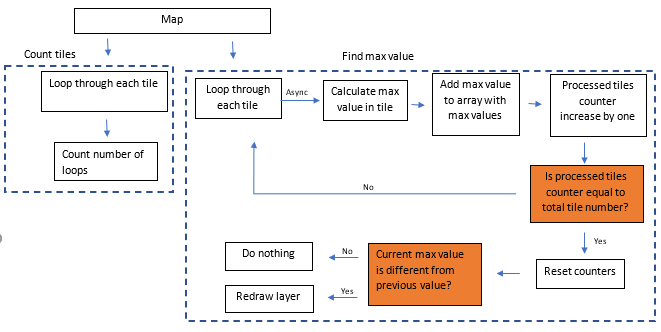
\includegraphics[width=.8\textwidth]{Pictures/DoubleLoop}
	\caption{Finding the largest value in all currently displayed tiles}
	\label{DoubleLoop}
\end{figure}

\section{Recolor when the max value change}

The recoloring function was already part of olGeoTiff. However, in Bernhard Baumrocks’ thesis this recoloring was triggered manually by the user when changing the color sliders. In this project the changing of colors will trigger automatically. The function for recoloring the map have therefore been set up to trigger on the user stopping this changing the view. By not triggering before the map movement is finished a smoother user experience is ensured, since new tiles does not have to processed before the user is finished with interacting with the map. The recolor function is running through all of the code mentioned in the previous sections. 

\begin{lstlisting}[language=JavaScript, caption={The JavaScript in the project}, label= VoresJS,escapechar=|]
map.on("moveend", function() {
recolorMap()
});
});
\end{lstlisting}
\section{Polish}
In addition to the rendering of the raster in the map, some features were also added to improve the user experience.


\subsection{Two maps}

\begin{figure} [H]
	\centering
	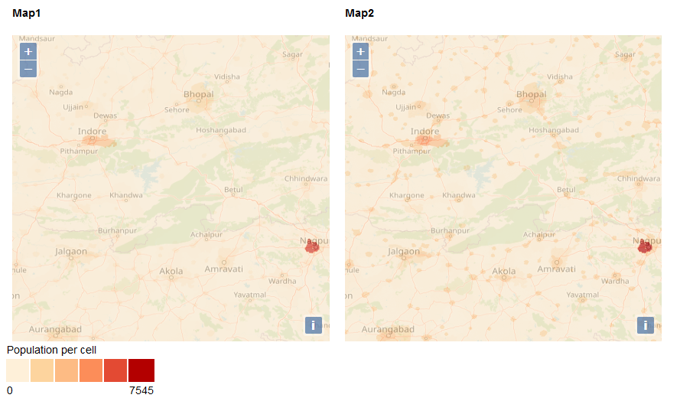
\includegraphics[width=.8\textwidth]{Pictures/DualMaps}
	\caption{A second map}
	\label{DualMaps}
\end{figure}
To be able to compare different rasters with eachother a second map was added as illustrated in figure \ref{DualMaps}. This second map is having its own raster dataset but sharing the view with the first map. This means that the two maps would always show the same area. Panning or zooming in one map would do the same action in the other map. The two maps are sharing the same legend. 

TODO: Write about evaluating max value based on two maps
%Add to dualmaps how the double evaluation for multiple maps were build 

\subsection{Search function}
In order to be able to faster navigate the map a search function was created as shown in figure \ref{SearchBar}. 

\begin{figure} [H]
	\centering
	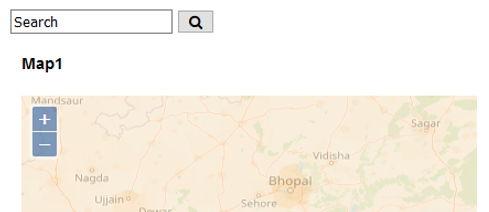
\includegraphics[width=.8\textwidth]{Pictures/SearchBar}
	\caption{A searchbar}
	\label{SearchBar}
\end{figure}

The user can use this to change the current view of the maps to a given location. This is accomplished through the help of Nominatim. This tool can search through Openstreetmap data by location names. It then returns data about the searched location. 

Among this data is the latitude and longitude for the central point of the place. \citep{Nominatim}
This coordinate is then used as the coordinate for the center of the map.
